\documentclass[11pt]{article}
\newcommand{\coursedocname}{Problem Set 4}

\usepackage[utf8]{inputenc}
\usepackage[T1]{fontenc}
\usepackage{lmodern}
\usepackage[margin=1in]{geometry}
\usepackage[dvipsnames]{xcolor}
\usepackage{graphicx, booktabs, enumitem, float, framed, caption, multirow}
\usepackage{fancyhdr}
\usepackage{tcolorbox}
\usepackage{listings}
\usepackage{tikz}
\usepackage{setspace}
\usepackage{needspace}
\IfFileExists{algorithm.sty}{%
  \usepackage{algorithm}
  \usepackage[noend]{algpseudocode}
  \newcommand{\hasalgorithms}{}%
}{}
\usepackage{amsmath,amssymb,bm,xcolor}






\usepackage{hyperref}

\definecolor{DartmouthGreen}{HTML}{00693E}
\newcommand{\dgreen}[1]{\textcolor{DartmouthGreen}{#1}}
\newcommand{\dgbf}[1]{\textbf{\dgreen{#1}}}      %
\urlstyle{same}
\hypersetup{
    colorlinks=true,
    linkcolor=DartmouthGreen,
    filecolor=DartmouthGreen,
    citecolor=DartmouthGreen,
    urlcolor=DartmouthGreen,
    breaklinks=true
}

\newcommand{\coursenumber}{COSC 81/281}
\newcommand{\courseterm}{Fall 2026}
\newcommand{\gradescopelink}{\textbf{Gradescope} (\url{https://www.gradescope.com/courses/1372528})}

\newcommand{\examDate}{Thursday, October 29 (in class)}
\newcommand{\psFourDue}{Monday, October 26 (11:59pm ET)}

\setlength{\parindent}{0pt}
\setlength{\parskip}{6pt plus 2pt minus 1pt}
\setlength{\headheight}{13.6pt}
\setlength{\emergencystretch}{3em}
\providecommand{\tightlist}{\setlength{\itemsep}{0pt}\setlength{\parskip}{0pt}}
\setcounter{secnumdepth}{0}

\DeclareRobustCommand{\callout}[2][gray!10]{%
  \begin{tcolorbox}[left=8pt, arc=0pt, outer arc=0pt,
                    colframe=#1, colback=#1, coltext=black]#2\end{tcolorbox}}




\newcommand{\gradstar}{$\bigstar$~\textsf{\small (required for 281; optional for 81)}~}
\newcommand{\bonusq}{\textsf{\small\textbf{[Bonus]}}~}
\newcommand{\bonus}{\bonusq}

\newcommand{\setupheader}[1]{%
  \fancypagestyle{default}{%
      \lhead{#1}
      \chead{}
      \rhead{\textbf{\coursenumber}}
      \lfoot{}
      \cfoot{}
      \rfoot{\thepage}
      \renewcommand{\headrulewidth}{0.4pt}
      \renewcommand{\footrulewidth}{0.4pt}
  }
  \pagestyle{default}
  \fancypagestyle{plain}{\pagestyle{default}}
}
\newcommand{\setupexamheader}[1]{%
  \fancypagestyle{default}{%
      \lhead{#1}
      \chead{Name:}
      \rhead{}
      \lfoot{}
      \cfoot{}
      \rfoot{\thepage}
      \renewcommand{\headrulewidth}{0.4pt}
      \renewcommand{\footrulewidth}{0.4pt}
  }
  \pagestyle{default}
  \fancypagestyle{plain}{\pagestyle{default}}
}
\newcommand{\pstitle}[2]{%
  \title{\textbf{\coursenumber:} #1}
  \author{\textbf{Due} #2\\
  }
  \date{}
}

\newcommand{\coursenotice}{%
  \callout{Problem sets are graded \textbf{pass/fail on completion}, and
  there are no late days. The problem sets are where the learning happens,
  and they are the best available practice for the midterm and final exam.
  Submit to \gradescopelink\ and assign each question to a page in your
  submission. Questions are welcome on \dgbf{Slack}. Starred ($\bigstar$)
  questions are required for COSC 281 students and optional (ungraded) for
  COSC 81 students.}}

\lstset{
  language=python,
  basicstyle=\ttfamily,
  commentstyle=\color{BrickRed},
  stringstyle=\color{ForestGreen},
  showstringspaces=false,
  breaklines=true,
  breakatwhitespace=true,
  keywordstyle=\color{Purple},
  emph={def},
  emphstyle=\color{RoyalBlue}
}
\lstnewenvironment{itemlisting}[1][]
 {\mbox{}\vspace*{-\baselineskip}%
  \lstset{xleftmargin=\leftmargin, linewidth=\linewidth, #1}}
 {}

\makeatletter
\def\fps@figure{htbp}
\makeatother
\ifdefined\hasalgorithms
\fi

\newcommand{\docfooter}{\vfill\begin{tiny}Updated \today\end{tiny}}

\newenvironment{studentanswer}[1]
  {\par\medskip\noindent
   \begin{tcolorbox}[height from=#1 to 100cm, colback=white, colframe=gray!60,
     boxrule=0.6pt, arc=0pt, outer arc=0pt, left=7pt, right=7pt,
     top=7pt, bottom=7pt, title={Answer / work}, fonttitle=\small,
     coltitle=black, colbacktitle=gray!8, titlerule=0pt]
   \ignorespaces}
  {\end{tcolorbox}\par}

\setupheader{\coursenumber\ -- \courseterm\ -- \coursedocname}

\begin{document}
\pstitle{Problem Set 4: Perception and Learning}{\psFourDue}
\maketitle

\coursenotice

\textbf{PS4 accepts no late submissions. Solutions release the same evening
the assignment is due (\psFourDue), so that you have them in hand while you
prepare for the exam (\examDate). Submit what you have by the deadline.}

\begin{quote}\small\textbf{AI Policy.} You may use any AI tools you like to assist you with your assignments, and you should, as that is likely how you will work for the rest of your career.
That being said, the written portions are practice for the in-class midterm and exam, which are closed book and on paper. You should strive to answer these yourself and use AI as a tutor and not an oracle.
\end{quote}

\callout{Please include an AI Tool Disclosure Below \vspace{50pt}}

\raggedbottom
\Needspace{5cm}
\textbf{What to submit.} Submit to \gradescopelink:
\begin{enumerate}\tightlist
\item \textbf{Written work (PDF).} Include your Part 1 answers, the Sobel
figure from Task 1, and the image comparison and explanation from Task 2.
P1(d) and P4(b) are graduate-only. You may write on this
handout or use \texttt{ps4/handout.tex}, entering answers in the
\texttt{studentanswer} blocks after each \texttt{SOLUTION HERE} marker.
Assign each question to its page or pages when uploading.
\item \textbf{Code.} Submit only \texttt{conv.py}. Run
\texttt{python ps4/code/autograder.py} from the course repository root.
The color experiment uses provided code and has no autograder submission.
\end{enumerate}
\clearpage
\section{Part 1: Written problems}
Show your calculations or explain your reasoning in each response area.
The written questions can be answered without running the programming tasks.

\subsection*{P1: Convolution and image boundaries}
The matrix $K$ is a filter, and $I$ is a grayscale image whose entries
are pixel intensities.
\[
K=\frac1{16}\begin{bmatrix}1&2&1\\2&4&2\\1&2&1\end{bmatrix},
\qquad
I=\begin{bmatrix}4&4&4\\4&12&4\\4&4&4\end{bmatrix}.
\]
Apply the filter by multiplying each entry of $K$ by the image entry
in the same position of the current $3\times3$ patch, then summing
the nine products. Use stride 1, meaning that consecutive filter
positions differ by one pixel. Fill each response grid with the
requested pixel values, and show your calculations below it. Leave
noninteger results as fractions.
\begin{enumerate}[label=(\alph*)]
\item \begin{minipage}[t]{\linewidth} With no padding, the filter fits in exactly one location.
Compute the convolution output by multiplying corresponding entries
and adding the nine products.

\begin{studentanswer}{3.5cm}
%%%%% SOLUTION HERE %%%%%
\begin{center}
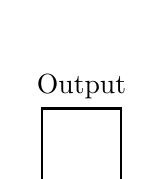
\begin{tikzpicture}
\draw[thick] (0,0) rectangle (1,1);
\node[above] at (.5,1){Output};
\end{tikzpicture}
\end{center}
\end{studentanswer}

\end{minipage}
\item \begin{minipage}[t]{\linewidth} Padding means adding entries around the image boundary before
applying the filter. Add one row or column of zeros on each of the four
sides of $I$. Fill every cell of the $5\times5$ grid with the resulting
padded image, including the zeros. Do not apply the filter yet.

\begin{studentanswer}{5cm}
%%%%% SOLUTION HERE %%%%%
\begin{center}
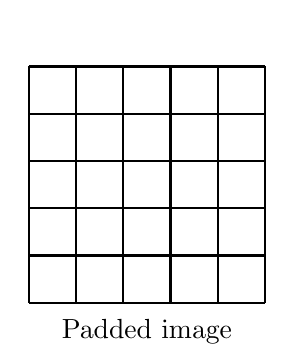
\begin{tikzpicture}[scale=.6]
\draw[step=1,thick] (0,0) grid (5,5);
\node[below] at (2.5,-.15){Padded image};
\end{tikzpicture}
\end{center}
\end{studentanswer}

\end{minipage}
\end{enumerate}
\clearpage
\noindent\textbf{P1 (continued)}
\begin{enumerate}[label=(\alph*),start=3]
\item \begin{minipage}[t]{\linewidth} Using the padded image from part (b), compute the output at the
top-left corner. Show the nonzero products in that weighted sum.
State the center output as well. Does it change from part (a)?
You do not need to compute the other seven output entries.

\begin{studentanswer}{5cm}
%%%%% SOLUTION HERE %%%%%
\begin{center}
\begin{tabular}{c|c|c}
 & Top-left output & Center output\\\hline
Value & &\\\hline
\end{tabular}
\end{center}
\end{studentanswer}

\end{minipage}
\item \begin{minipage}[t]{\linewidth} \gradstar Suppose the border is instead filled by repeating the nearest
original pixel value. Explain which output entries can change and why.
Why is the choice of padding an assumption about the image, rather than
only a way to control the output size? No additional calculation is required.

\begin{studentanswer}{4cm}
%%%%% SOLUTION HERE %%%%%
\end{studentanswer}

\end{minipage}
\end{enumerate}

\clearpage
\subsection*{P2: What does a filter detect?}
The figure shows one grayscale image and two filtered outputs, A and B.
The two filters are
\[
K_1=\begin{bmatrix}-1&0&1\\-2&0&2\\-1&0&1\end{bmatrix},
\qquad K_2=\frac19\begin{bmatrix}1&1&1\\1&1&1\\1&1&1\end{bmatrix}.
\]
Each output is displayed using the magnitude of its values, scaled so
that its largest magnitude is white. Focus on which image features
remain visible rather than comparing brightness between panels.
\begin{center}
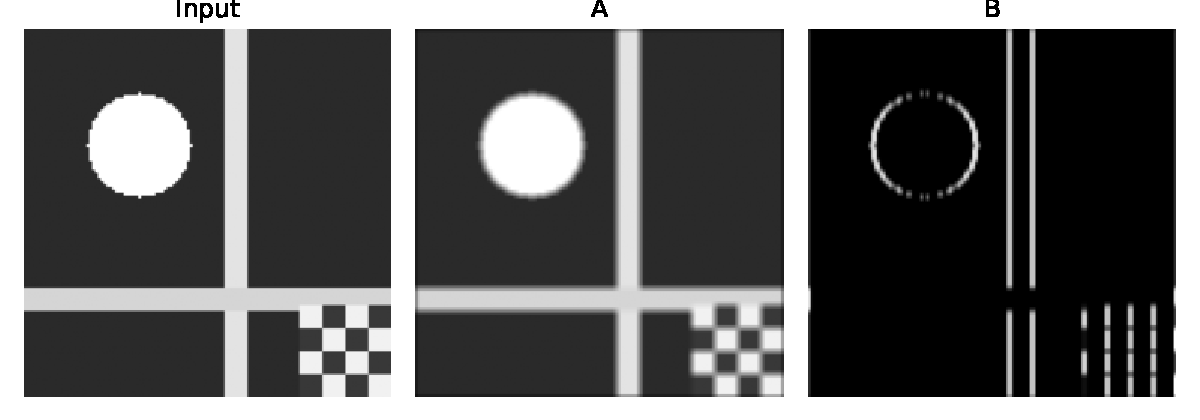
\includegraphics[width=.9\linewidth]{ps4/figures/kernel_pair.pdf}
\end{center}
\begin{enumerate}[label=(\alph*)]
\item \begin{minipage}[t]{\linewidth} Match each filter to output A or B and explain both choices.
For $K_1$, compare the left and right coefficients on a constant patch
and on a patch whose right side is brighter. For $K_2$, use the fact
that its positive coefficients sum to one. Explain what happens at an edge.

\begin{studentanswer}{6cm}
%%%%% SOLUTION HERE %%%%%
\end{studentanswer}

\end{minipage}
\end{enumerate}

\clearpage
\subsection*{P3: Following an image through a network}
A grayscale image stores one intensity at each pixel. A \emph{channel}
is one grid of values over the image. Thus an $8\times8$ grayscale image
has height 8, width 8, and one channel. An RGB image has three such grids,
one each for red, green, and blue. The input in this question is grayscale.

A convolutional layer applies several learned filters to the same input.
Each filter produces its own grid of responses, called an output channel.
These learned channels need not represent colors. One might respond to
an edge, while another responds to a different pattern. Here the layer
uses two $3\times3$ filters, stride 1, and one pixel of zero padding on
every side. Each filter combines one input patch into one output value.

\emph{Max pooling} is a separate layer applied after the convolution.
It divides each channel into nonoverlapping $2\times2$ blocks and
replaces each block by its largest value. For example,
$\begin{bmatrix}1&5\\3&2\end{bmatrix}$ becomes the single value 5.
It processes each channel independently and has no learned parameters.
\begin{enumerate}[label=(\alph*)]
\item \begin{minipage}[t]{\linewidth} Start with the $8\times8\times1$ input. After padding, each
spatial dimension is 10. A width-3 filter fits at $10-3+1$ horizontal
positions, and the same count applies vertically.
Fill the table with the dimensions after convolution and after pooling.
The number of convolution channels equals the number of filters.
Pooling halves each spatial dimension but keeps the channels separate.

\begin{studentanswer}{4.5cm}
%%%%% SOLUTION HERE %%%%%
\begin{center}
\renewcommand{\arraystretch}{1.4}
\begin{tabular}{l|c|c|c}
Layer & Height & Width & Channels\\\hline
Convolution & & &\\\hline
Max pooling & & &\\\hline
\end{tabular}
\end{center}
\end{studentanswer}

\end{minipage}
\end{enumerate}
\clearpage
\noindent\textbf{P3 (continued)}
\begin{enumerate}[label=(\alph*),start=2]
\item \begin{minipage}[t]{\linewidth} Practice max pooling on the following $4\times4$ portion of one
channel. Use nonoverlapping $2\times2$ blocks and write the four maxima
in the output grid. State one kind of information lost by this operation.
\[
\begin{bmatrix}1&5&2&0\\3&2&4&1\\0&7&3&8\\6&1&2&5\end{bmatrix}
\]

\begin{studentanswer}{4.5cm}
%%%%% SOLUTION HERE %%%%%
\begin{center}
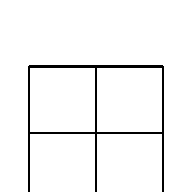
\begin{tikzpicture}[scale=.85]
\draw[step=1,thick] (0,0) grid (2,2);
\end{tikzpicture}
\end{center}
\end{studentanswer}

\end{minipage}
\item \begin{minipage}[t]{\linewidth} A \emph{fully connected layer} uses every value from the preceding
layer as an input to each of its outputs. First, place the pooled
$4\times4\times2$ values in a list $x_1,\ldots,x_N$. This rearrangement
is called flattening and adds no learned parameters. The layer has
three outputs, each computed as
\[
y_j=w_{j1}x_1+\cdots+w_{jN}x_N+b_j,\qquad j=1,2,3.
\]
Here each weight $w_{ji}$ and each bias $b_j$ is a learned number.
Find $N$, then count the weights and biases for one output and for
all three outputs. Count only this fully connected layer.

\begin{studentanswer}{4cm}
%%%%% SOLUTION HERE %%%%%
\end{studentanswer}

\end{minipage}
\end{enumerate}

\clearpage
\subsection*{P4: Evaluating an imitation policy}

A team trains a steering policy for the Dubins car using behavior cloning.
The training data contain observations and steering commands from
successful expert laps of a slalom course. The learned policy passes the
first two gates, then drifts wide on the third. Its steering becomes
progressively less effective until it leaves the course. The demonstrations
contain no examples of recovering from this deviation.

\begin{enumerate}[label=(\alph*)]

\item \begin{minipage}[t]{\linewidth}
Identify a learning-related cause of this failure. In two or three
sentences, explain why the errors can grow during a rollout even when
the policy predicts steering accurately on held-out expert data.

\begin{studentanswer}{3.5cm}
%%%%% SOLUTION HERE %%%%%

\end{studentanswer}

\end{minipage}

\item \begin{minipage}[t]{\linewidth} \gradstar Suppose collecting additional expert demonstrations is not
possible. Propose one modification that could reduce failures during
deployment. Explain why it could help and identify one limitation. Answer
in two or three sentences. Multiple answers may be acceptable when their
assumptions are stated and justified.

\begin{studentanswer}{4cm}
%%%%% SOLUTION HERE %%%%%
\end{studentanswer}

\end{minipage}
\end{enumerate}

\clearpage
\section{Part 2: Image filtering experiments}
Run all commands from the course repository root with the course Python
environment active. The only file to implement and submit is
\texttt{ps4/code/conv.py}. Task 2 uses a complete, provided program.

\subsection{Task 1: Convolution and Sobel}
A grayscale image is a two-dimensional array with shape $(H,W)$.
Each entry is an intensity. A filter is a smaller array that assigns
weights to a local image patch. At each position, multiply entries
in the same positions of the patch and filter, then sum the products
to obtain one output value.

The file \texttt{conv.py} contains two functions to complete.
The image loader, grayscale conversion, filter coefficients, and plotting
are provided. You do not need to edit any other file.
\begin{enumerate}
\item In \texttt{convolve2d(image, kernel, pad=0, stride=1)}, convert
the input arrays to floating-point values with \texttt{np.asarray}.
The image has shape $(H,W)$ and the filter has odd square shape $(K,K)$.
\item Add \texttt{pad} rows or columns of zeros to each side of the
image using \texttt{np.pad}. The padded image has shape
$(H+2\,\texttt{pad},W+2\,\texttt{pad})$.
\item Allocate a floating-point output array with dimensions
\[
H_{\rm out}=(H+2\,\texttt{pad}-K)\mathbin{//}\texttt{stride}+1,\quad
W_{\rm out}=(W+2\,\texttt{pad}-K)\mathbin{//}\texttt{stride}+1.
\]
Here \texttt{//} is integer division. Stride gives the number of input
pixels between neighboring filter positions.
\item Use nested loops over output rows $i$ and columns $j$.
The corresponding patch starts at row
$r=i\,\texttt{stride}$ and column $c=j\,\texttt{stride}$ in the padded
image. Select it using \texttt{padded[r:r+K, c:c+K]}.
\item Multiply the patch and \texttt{kernel} entry by entry.
Use \texttt{np.sum} to store their weighted sum in output entry $(i,j)$.
Return the completed array. Do not use library filtering functions
from SciPy, OpenCV, or a neural-network framework.
\end{enumerate}

For a small check, an image
$\begin{bmatrix}1&2&3\\4&5&6\\7&8&9\end{bmatrix}$
with a $3\times3$ filter whose entries are all $1/9$, no padding, and
stride 1 should produce the single value 5. A $4\times4$ image with
a $3\times3$ filter and padding 1 should produce a $4\times4$ output
at stride 1 and a $2\times2$ output at stride 2.

\clearpage
\noindent\textbf{Task 1 (continued)}

\textbf{Sobel responses.} The supplied \texttt{SOBEL\_X} filter compares
intensities to the left and right of each pixel. \texttt{SOBEL\_Y}
compares intensities above and below it. They produce signed responses
$g_x$ and $g_y$, which indicate local intensity changes in the two
directions. Large response magnitudes often occur along visible edges.
Complete \texttt{sobel(image)} as follows.
\begin{enumerate}
\item Call your \texttt{convolve2d} with \texttt{SOBEL\_X},
padding 1, and stride 1 to obtain $g_x$.
\item Call it again with \texttt{SOBEL\_Y} and the same padding and stride
to obtain $g_y$.
\item Compute $\sqrt{g_x^2+g_y^2}$ separately at every pixel using
NumPy array operations. Return \texttt{gx, gy, magnitude}.
All three arrays must have the same shape as the input image.
\end{enumerate}
Run
\begin{center}
\texttt{python ps4/code/conv.py}\\
\texttt{python ps4/code/autograder.py}
\end{center}
The first command loads the supplied simulator image, converts it to
grayscale, calls your functions, and saves
\texttt{ps4/code/plots/edges.png}. The second command runs the public
checks. Submit only \texttt{conv.py} to the autograder.

\textbf{PDF response.} Include \texttt{edges.png} and identify one boundary
that produces a strong response. No additional code or written derivation
is required.

\begin{studentanswer}{8cm}
%%%%% SOLUTION HERE %%%%%
\end{studentanswer}

\clearpage
\subsection{Task 2: Color and illumination}
This experiment uses \texttt{ps4/code/hsv\_detector.py}, which is fully
implemented. You do not need to write a detector or submit code for this task.

\textbf{Grayscale, RGB, and HSV.} A grayscale image stores one intensity
per pixel. An RGB image stores three values per pixel, for red, green,
and blue, so its array has shape $(H,W,3)$. Those three channels together
describe a color. Converting RGB to grayscale combines them into one
intensity and discards some color information.

HSV is another representation of the same RGB color, not a new sensor.
Hue describes the color family and is represented here by an angle in
$[0,360)$. Saturation describes how far the color is from gray, and value
describes its brightness. Both lie in $[0,1]$ in the provided code.
HSV separates these quantities for thresholding, but it does not make
colors invariant to illumination or camera settings. Hue is especially
unreliable when saturation is very low.

\textbf{Provided detector.} The program converts each image to HSV and
selects pixels whose hue, saturation, and value meet fixed thresholds.
It then keeps the largest connected region of selected pixels.
The colored overlay shows that region, and a marker shows its center.
This is a color rule, not a shape recognizer. A similarly colored
background can be selected instead of the object.

\begin{enumerate}
\item Run \texttt{python ps4/code/hsv\_detector.py}.
The program uses the supplied simulator images and saves overlays in
\texttt{ps4/code/plots/}. Open them to see which pixels the rule selects.
\item Choose a red, orange, or yellow object and photograph the same
object in two lighting conditions, such as daylight and warm indoor
light, or ordinary light and strong shadow. Keep the detector thresholds
fixed. The exercise concerns the change in appearance, not whether the
object is literally a cone.
\item Transfer the photos to the computer running your code.
Create a folder named \texttt{photos} inside \texttt{ps4/code/}, then
copy the files there using your file manager. If your code runs in a
hosted notebook, use its file browser's upload button and place the
files in that same folder. Use JPEG or PNG images. Export HEIC phone
photos as JPEG or PNG first.
\item Rename the files \texttt{daylight.jpg} and \texttt{indoor.jpg},
or substitute their actual names in this command:
\begin{center}
\texttt{python ps4/code/hsv\_detector.py}\\
\texttt{ps4/code/photos/daylight.jpg ps4/code/photos/indoor.jpg}
\end{center}
Enter the two displayed lines as one command. Put quotation marks
around any path containing spaces. The program prints each output path.
\end{enumerate}
If taking or transferring photos is not possible, run
\texttt{python ps4/code/hsv\_detector.py --lighting-demo}.
It uses a supplied simulator frame to create controlled dim and
color-shifted examples, then applies the same detector. These are
synthetic changes, not measurements of a real camera.
Use the original and one changed image, and state that you used this option.

\clearpage
\noindent\textbf{Task 2 responses}
\begin{enumerate}[label=(\alph*)]
\item Include the two overlays you compared and label their lighting
conditions. State whether they are your photographs or the provided
synthetic lighting examples.

\begin{studentanswer}{9cm}
%%%%% SOLUTION HERE %%%%%
\end{studentanswer}

\item In a short paragraph, explain how the appearance and selected
region changed. Relate one observation to brightness, saturation,
color, shadows, or white balance. What does the comparison show about
the limits of using fixed color thresholds? Successful detection in
both images is also a valid result.

\begin{studentanswer}{5cm}
%%%%% SOLUTION HERE %%%%%
\end{studentanswer}

\end{enumerate}
\docfooter
\end{document}
